\documentclass[10pt,aspectratio=149]{beamer}

\usecolortheme{Calm}
\usetheme{Calm}

%%\usepackage{minted}
%%\usemintedstyle{pastie}

\usepackage{pgfplots}
\usepackage{pgfplotstable}
\usepackage[utf8]{inputenc}
\usetikzlibrary{shapes, arrows, positioning}

\setbeamertemplate{itemize items}[circle]

\usepackage[font=footnotesize,skip=3pt]{caption}
\captionsetup[figure]{labelformat=empty}
\captionsetup[table]{labelformat=empty}
\setbeamerfont{alerted text}{series=\bfseries}

\author{Steve Vissault, Matthew Talluto, \\
Isabelle Boulangeat and Dominique Gravel}
\title{Difficult migration of temperate tree species \\
in the boreal forest under climate change?}
\date{\today}
\institute{Université du Québec à Rimouski}


\begin{document}
\begin{frame}[plain]
   \titlepage
\end{frame}

%%% Keys
%1. Le titre
%2. Travail collaboratif qui regroupe plusieurs chercheurs du laboratoire d'écologie théorique de dominiaue gravel
%3. Fruit de 1 ans de travail dans le cadre de ma maitrise
%4. Cette présentation a pour objectif de montrer quelques résultats préliminaires

%%%%%%%%%%%%%%%%%%%%%%%%%%%%%%%%%%%%%%%%%%%%%%%%%%%%%%%%%%%%%%%%%%%%%%%%%%%%%%%%%%%%%%%%%%%%%%%%
%%% Context

\begin{frame}{Context}{The boreal-temperate ecotone}

The surface of the boreal-temperate forests ecotone is \textbf{expected to shift over the next 100 years}.

\begin{figure}
	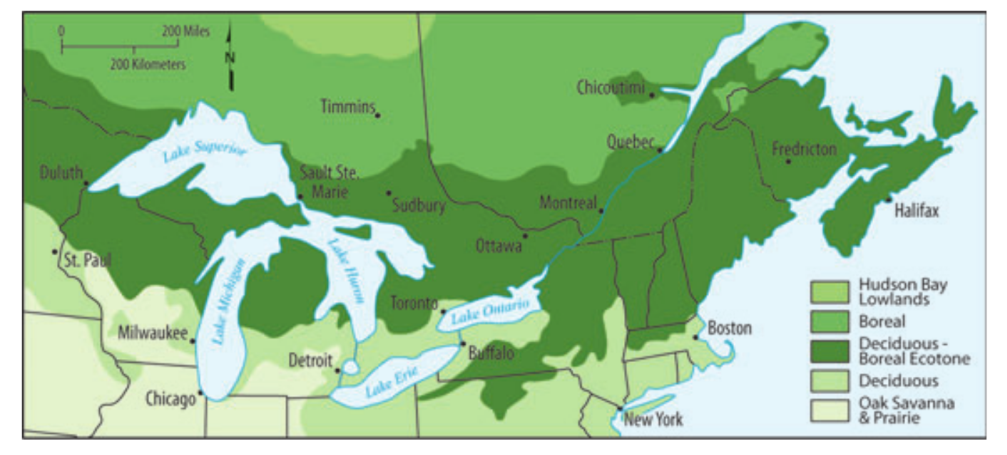
\includegraphics[width=.70\paperwidth]{Figs/ecotone.pdf}
\end{figure}

   \paper{Goldblum and Rig, 2010}
\end{frame}

%% 


%%%%%%%%%%%%%%%%%%%%%%%%%%%%%%%%%%%%%%%%%%%%%%%%%%%%%%%%%%%%%%%%%%%%%%%%%%%%%%%%%%%%%%%%%%%%%%%%
%%% Context

\begin{frame}{Context}{The boreal-temperate ecotone}

1. The location of this ecotone is \textbf{responsive to climate}.

\begin{figure}
	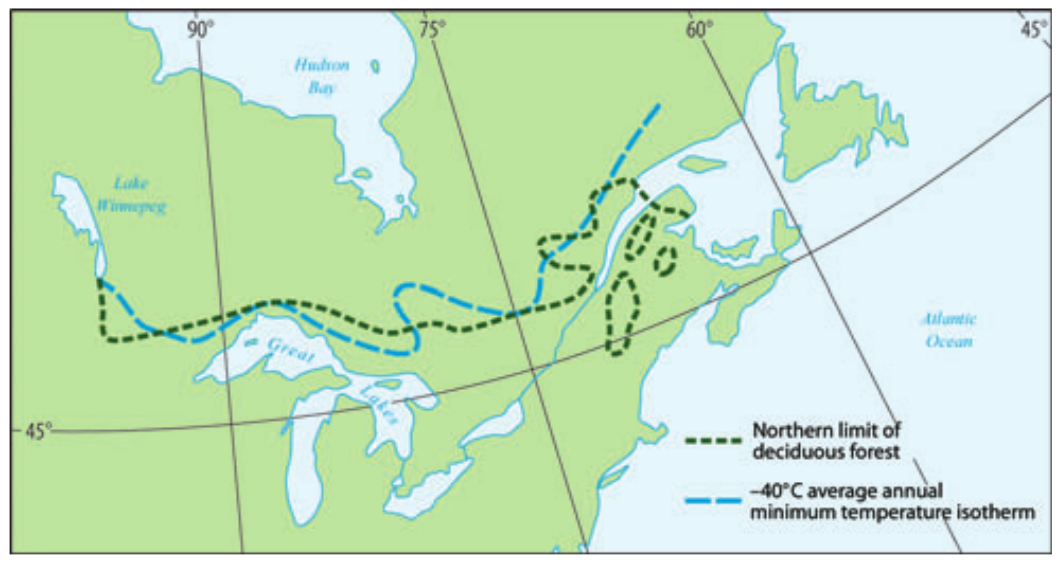
\includegraphics[width=.70\paperwidth]{Figs/climecotone.png}
\end{figure}

   \paper{Goldblum and Rig, 2010}
\end{frame}

%%%%%%%%%%%%%%%%%%%%%%%%%%%%%%%%%%%%%%%%%%%%%%%%%%%%%%%%%%%%%%%%%%%%%%%%%%%%%%%%%%%%%%%%%%%%%%%%
%%% SDM

\begin{frame}{Context}{Predicted future species distribution}

2. Several temperate forest species are predicted to \textbf{shift northward} under climate change
	\vspace{-1.75em}
	  \begin{columns}[t]
        \centering

        \begin{column}{0.45\linewidth}
	        \centering
	        \begin{figure}
	          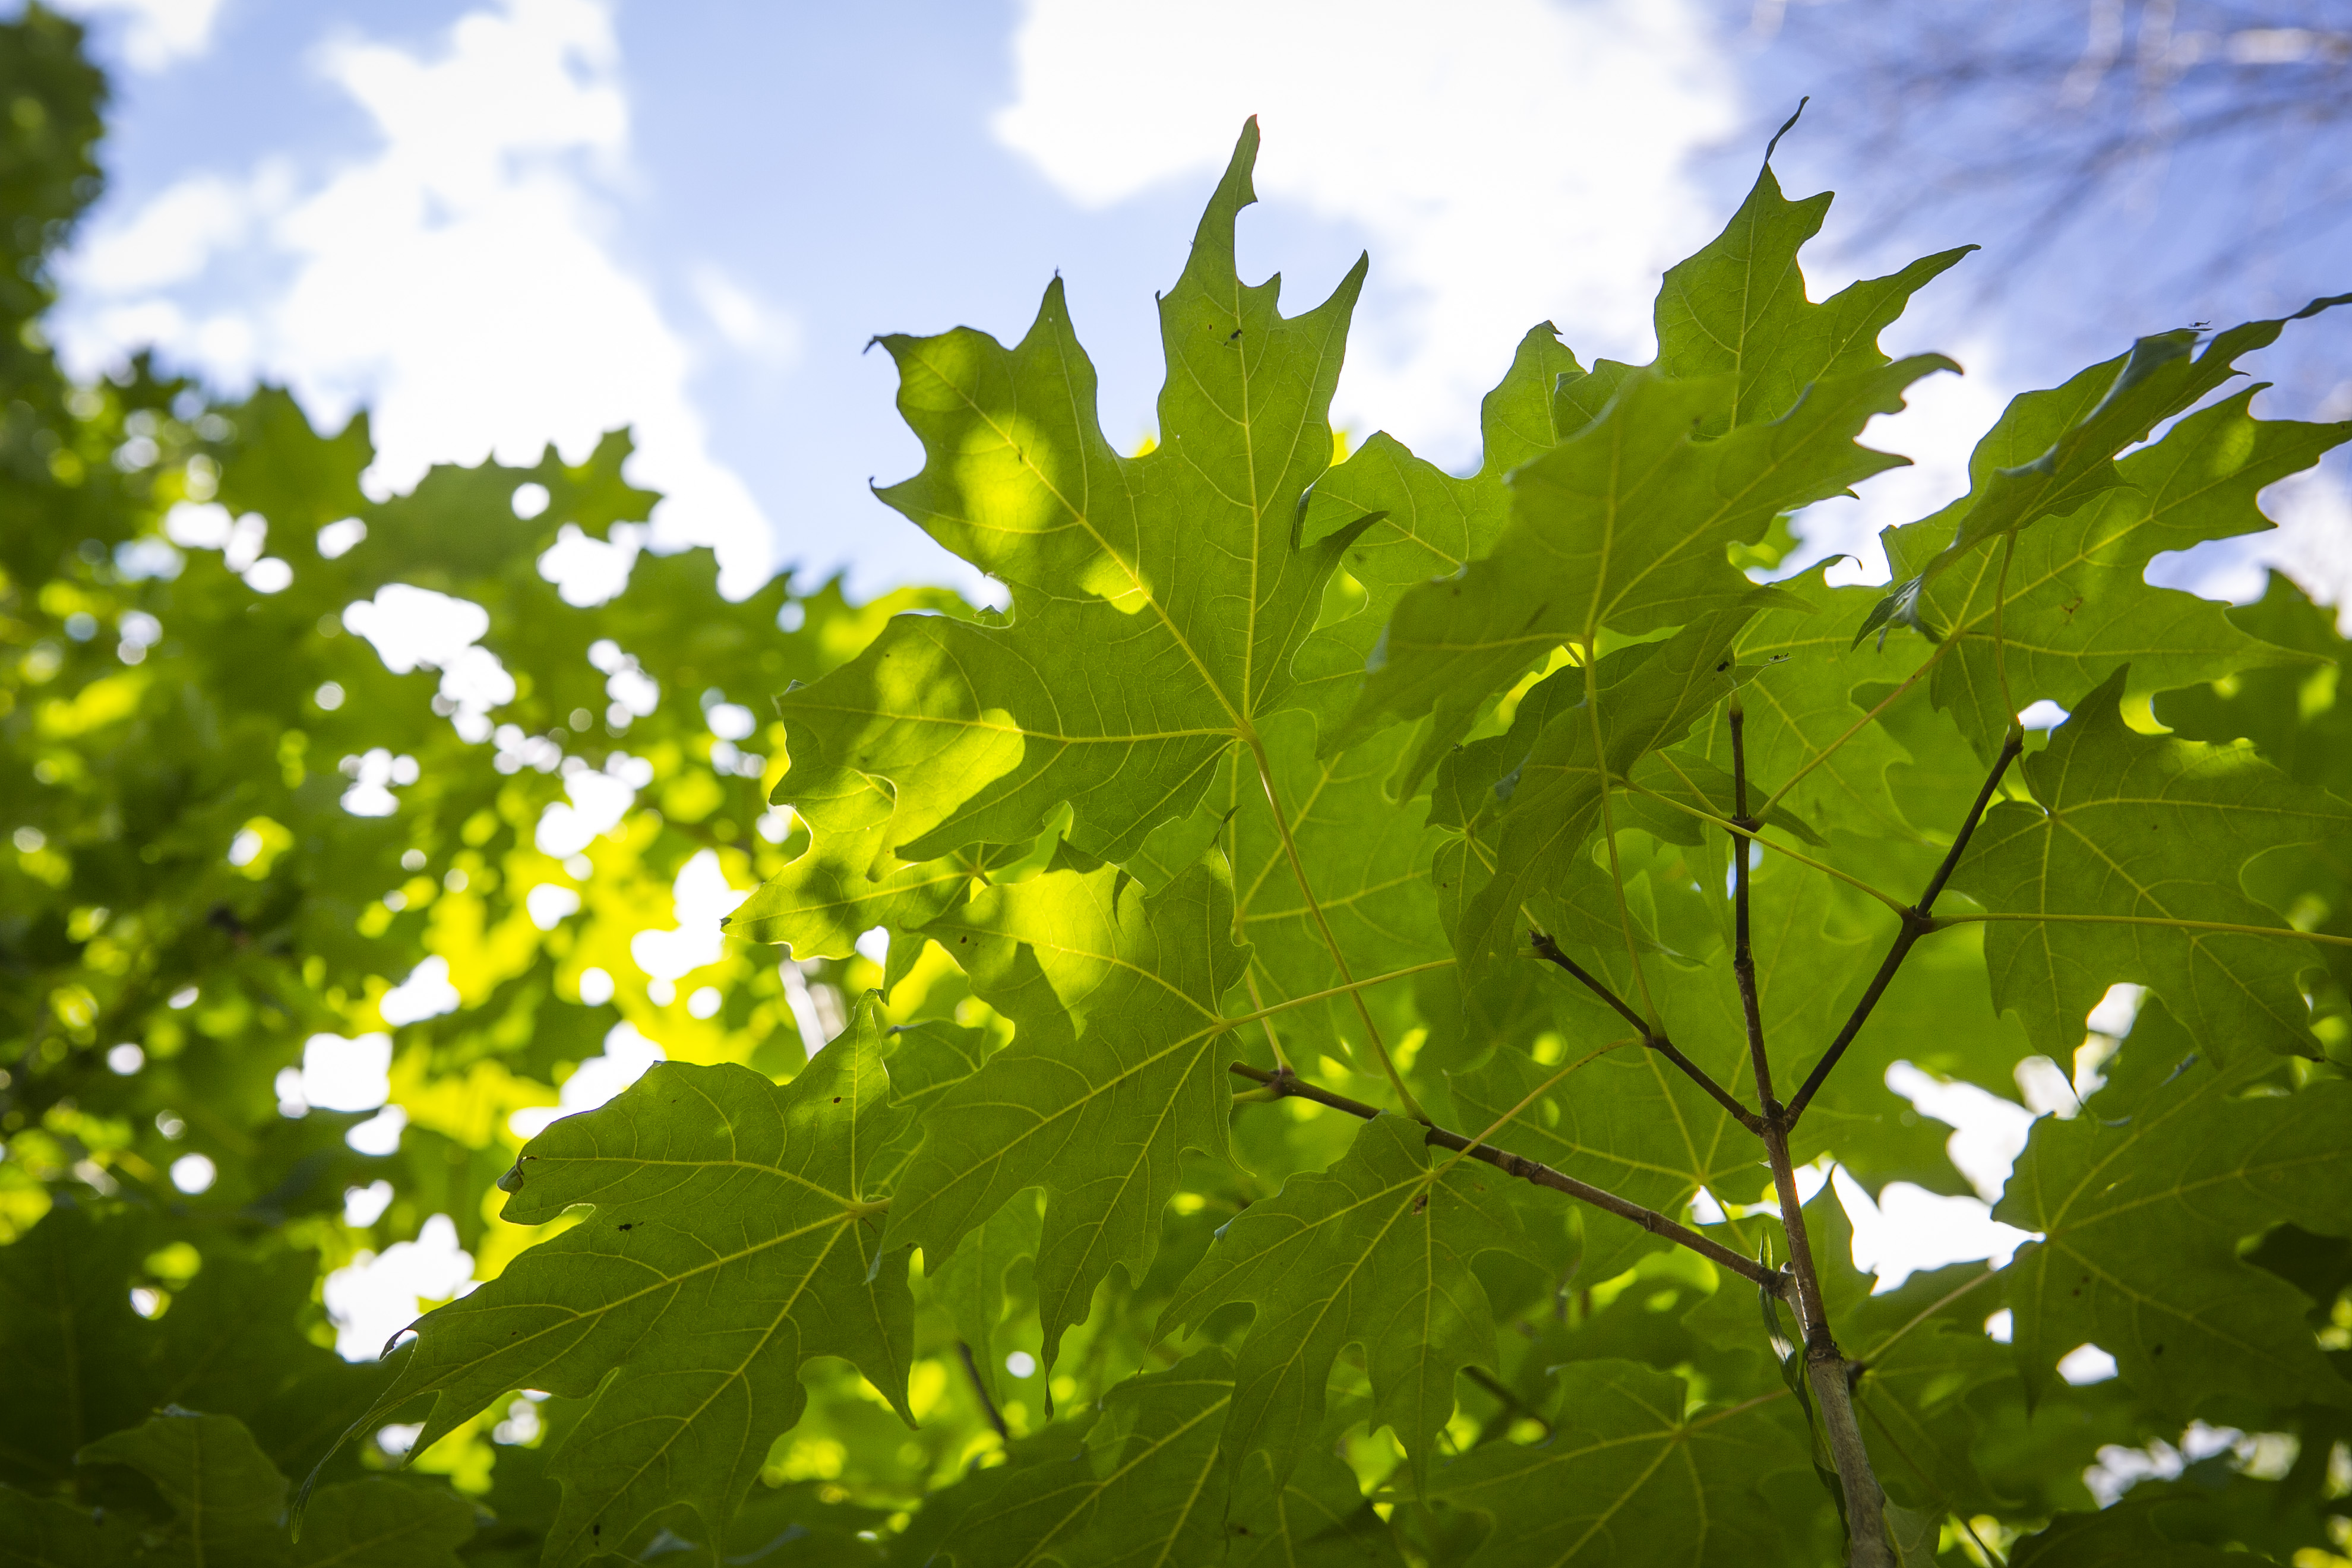
\includegraphics[width=0.75\linewidth]{Figs/sugar.jpg}
	          \caption{\textbf{Sugar maple}}
	          \vspace{-2.5em}
	        \end{figure}
	         \pause
	        \begin{figure}
	          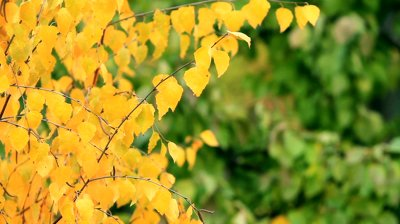
\includegraphics[width=0.75\linewidth]{Figs/birch.jpg}
	          \caption{\textbf{Yellow birch}}
	          \vspace{-2.5em}
	        \end{figure}
        \end{column}

        \begin{column}{0.45\linewidth}
	        \centering
			\pause
	        \begin{figure}
	          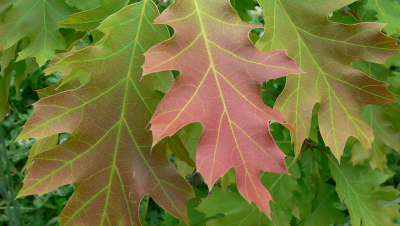
\includegraphics[width=0.75\linewidth]{Figs/oak.jpg}
	          \caption{\textbf{Red oak}}
	          \vspace{-2.5em}
	        \end{figure}
	       	\pause
	        \begin{figure}
	          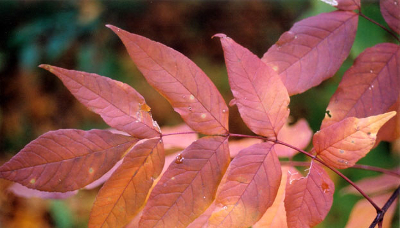
\includegraphics[width=0.75\linewidth]{Figs/ash.jpg}
	          \caption{\textbf{American ash}}
	          \vspace{-2.5em}
	        \end{figure}
        \end{column}
      \end{columns}



   \paper{McKenney \textit{et al}, 2007; Woodall \textit{et al}, 2008; Iverson and Prasad, 2002. Web illustrations}
\end{frame}

%%% SDM are limited in this study context
% Centered on species
% Abiotic conditions (e.g. Climate, soil)
% Spatially implicit
% Instantaneous dynamic
			  
%%%%%%%%%%%%%%%%%%%%%%%%%%%%%%%%%%%%%%%%%%%%%%%%%%%%%%%%%%%%%%%%%%%%%%%%%%%%%%%%%%%%%%%%%%%%%%%%
%%% SDM

\begin{frame}{Context}{Predicted future species distribution}

2. Several temperate forest species are predicted to \textbf{shift northward} under climate change

	\begin{figure}
		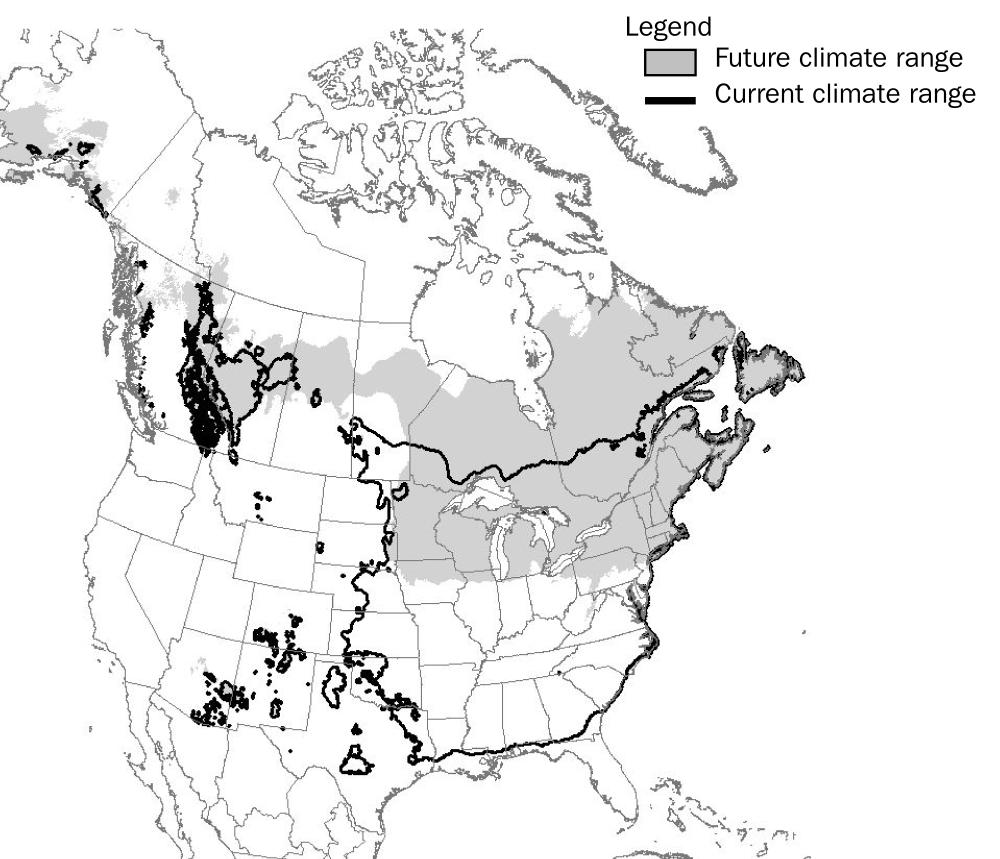
\includegraphics[width=.40\paperwidth]{Figs/sugar_map_distrib.jpg}
	\caption{ \textbf{Future climate enveloppe of Sugar maple (2071-2100)}}
	\end{figure}

   \paper{McKenney \textit{et al}, 2007}

\end{frame}

%%% SDM are limited in this study context
% Centered on species
% Abiotic conditions (e.g. Climate, soil)
% Spatially implicit
% Instantaneous dynamic

%%%%%%%%%%%%%%%%%%%%%%%%%%%%%%%%%%%%%%%%%%%%%%%%%%%%%%%%%%%%%%%%%%%%%%%%%%%%%%%%%%%%%%%%%%%%%%%%
%%% Tool

%%% Quand on s'intéresse au changements d'aire de répartition d'un communauté, deux processus sont à prendre en considérations:
\begin{frame}{Context}{Limits and difficulties in this study context}

\textbf{Forest have:}
		\begin{enumerate}
			\item Limited dispersions
			\item Slow population dynamics
			\item Successional stages (dynamic communities)
		\end{enumerate}
\vspace{1em}
\pause
\textbf{To predict species or communities range shift we need to include:}
	\begin{itemize}
		\item Spatial interactions (e.g. competition)
		\item Population demography
	\end{itemize}

	%% remplacer par titre des axes
	\pause
	\alert{These components will be effected by future climate}
  \paper{Travis \textit{et al}, 2013}
\end{frame}

%% Demographical process

%%%%%%%%%%%%%%%%%%%%%%%%%%%%%%%%%%%%%%%%%%%%%%%%%%%%%%%%%%%%%%%%%%%%%%%%%%%%%%%%%%%%%%%%%%%%%%%%
%%% Tools

\begin{frame}{Context}{Modelling compromise}
	
		\begin{figure}
			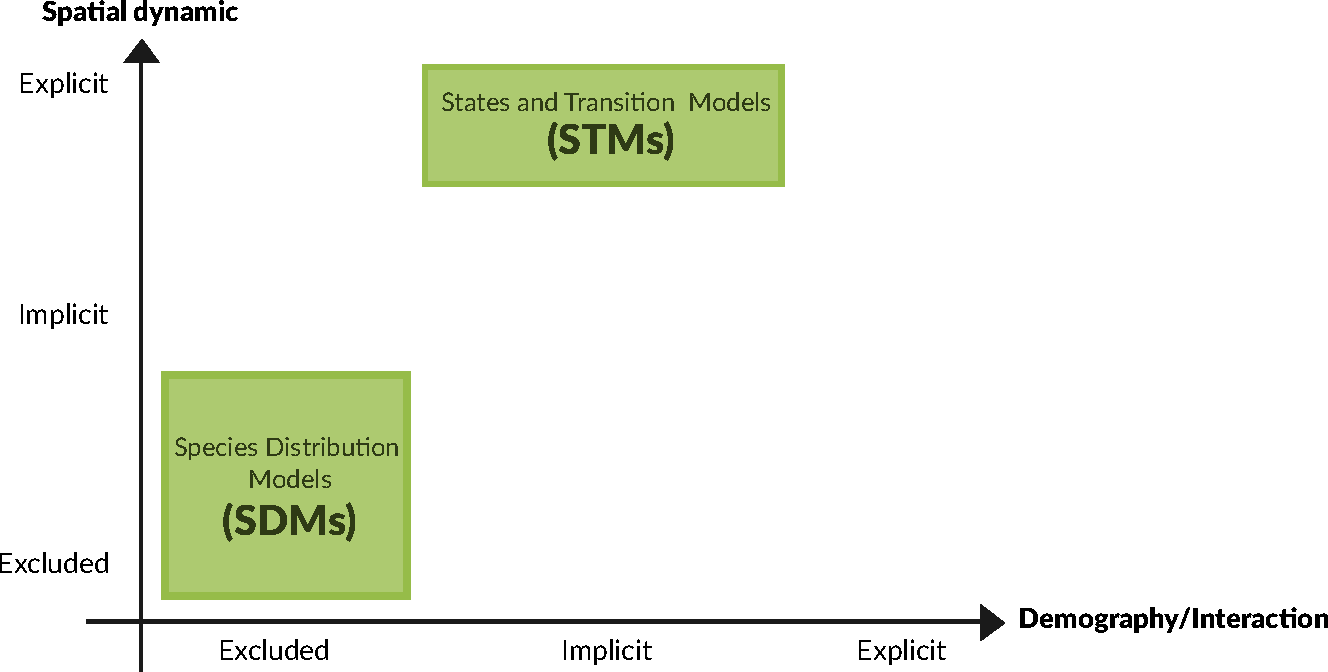
\includegraphics[width=1.2\paperheight]{Figs/schema_models.pdf}
		\end{figure}
\paper{Scheller and Mladenoff \textit{et al}, 2006; Kriticos \textit{et al}, 2013}
\end{frame}


%%%%%%%%%%%%%%%%%%%%%%%%%%%%%%%%%%%%%%%%%%%%%%%%%%%%%%%%%%%%%%%%%%%%%%%%%%%%%%%%%%%%%%%%%%%%%%%%
%%% Objective

%%% 1. L'un des objectifs de ce mémoire consiste à évaluer les changements dans l'aire de répartition de la communauté de la forêt nordique du Québec ainsi que son taux de migration sous l'effet des changements climatiques 

%%% 2. Lorsque l'on parle de migration et de changement d'aire de répartition d'une espèce dans ce cas-ci d'une communauté, on s'intéresse particulièrement à la distance et au de migration. 

%%% Carte domaine bioclimatique + renforcer dichotomie fonctionnement écosystème

\begin{frame}{Study ojective}

\textbf{Main objective:} Assess range shift and migration rates of the temperate forest community toward boreal forest under climate change.

\pause 

\vspace{1em}
\textbf{Why ?}
		\begin{itemize}
			\item Predict the future distribution of temperate species community in Quebec
		 	\item Improve and adapt our forests management practices under climate change
		\end{itemize}

\end{frame}

%%%%%%%%%%%%%%%%%%%%%%%%%%%%%%%%%%%%%%%%%%%%%%%%%%%%%%%%%%%%%%%%%%%%%%%%%%%%%%%%%%%%%%%%%%%%%%%%
%% Generality of the model 


\begin{frame}{New approach}{States and Transitions Model}

\begin{columns}[c]
	\begin{column}[c]{.40\paperwidth}
		\begin{figure}
			\small{\begin{center}

\tikzstyle{Temperate}=[circle,
    thick,
    minimum size = 1cm,
    inner sep =5pt,
    draw=Temperate,
    fill=Temperate]
\tikzstyle{Boreal}=[circle,
    thick,
    minimum size = 1cm,
    inner sep =5pt,
    draw=Boreal,
    fill=Boreal]
\tikzstyle{Regeneration}=[circle,
    thick,
    minimum size = 1cm,
    inner sep =5pt,
    draw=Regeneration,
    fill=Regeneration]
\tikzstyle{Mixed}=[circle,
    thick,
    minimum size = 1cm,
    inner sep =5pt,
    draw=Mixed,
    fill=Mixed]


\begin{tikzpicture}[->,>=stealth',auto,scale=0.45]
    \node [circle,Mixed] (M) at (0,0) {\color{white}\textbf{M}};
    \node [circle,Boreal] (B) at (-5,5) {\color{white}\textbf{B}};
    \node [circle,Temperate] (T) at (5,5) {\color{white}\textbf{T}};
    \node [circle,Regeneration] (R) at (0,10) {\color{white}\textbf{R}};

    \draw[thick,-latex] (M) to[bend right=10] node[above,sloped] {} (B);
    \draw[thick,-latex] (B) to[bend right=10] node[below,sloped] {} (M);

    \draw[thick,-latex] (T) to[bend right=10] node[above,sloped] {} (M);
    \draw[thick,-latex] (M) to[bend right=10] node[below,sloped] {} (T);

    \draw[thick,-latex] (T) to[bend right=10] node[above,sloped] {} (R);
    \draw[thick,-latex] (R) to[bend right=10] node[below,sloped] {} (T);

    \draw[thick,-latex] (R) to[bend right=10] node[above,sloped] {} (B);
    \draw[thick,-latex] (B) to[bend right=10] node[below,sloped] {} (R);

    \draw[thick,-latex,transform canvas={xshift=0.6ex}] (R) to node[above,sloped,rotate=90,transform canvas={xshift=1.5ex}] {} (M);
    \draw[thick,-latex,transform canvas={xshift=-0.6ex}] (M) to node[above,sloped,rotate=-90,transform canvas={xshift=-1.5ex}] {} (R);
\end{tikzpicture}
\end{center}

}
		\end{figure}
	\end{column}
	\begin{column}[l]{.50\paperwidth}
	\textbf{Model Description}
		\begin{itemize}
			\item Lanscape scale
			\item \textbf{4 States:}
			\begin{itemize}
				\item \textbf{B} Boreal forest
				\item \textbf{M} Mixed forest
				\item \textbf{T} Temperate forest
			\end{itemize}
			\item \textbf{R} corresponds to a post-disturbance patch
			\item Spatially explicit and stochastic model
		\end{itemize}
	\end{column}
\end{columns}
\end{frame}

%%%%%%%%%%%%%%%%%%%%%%%%%%%%%%%%%%%%%%%%%%%%%%%%%%%%%%%%%%%%%%%%%%%%%%%%%%%%%%%%%%%%%%%%%%%%%%%%
%% Generality of the model 

\begin{frame}{New approach}{States and Transitions Model}

\begin{columns}[c]
	\begin{column}[c]{.40\paperwidth}
		\begin{figure}
			\small{\begin{center}

\tikzstyle{Temperate}=[circle,
    thick,
    minimum size = 1cm,
    inner sep =5pt,
    draw=Temperate,
    fill=Temperate]
\tikzstyle{Boreal}=[circle,
    thick,
    minimum size = 1cm,
    inner sep =5pt,
    draw=Boreal,
    fill=Boreal]
\tikzstyle{Regeneration}=[circle,
    thick,
    minimum size = 1cm,
    inner sep =5pt,
    draw=Regeneration,
    fill=Regeneration]
\tikzstyle{Mixed}=[circle,
    thick,
    minimum size = 1cm,
    inner sep =5pt,
    draw=Mixed,
    fill=Mixed]


\begin{tikzpicture}[->,>=stealth',auto,scale=0.45]
    \node [circle,Mixed] (M) at (0,0) {\color{white}\textbf{M}};
    \node [circle,Boreal] (B) at (-5,5) {\color{white}\textbf{B}};
    \node [circle,Temperate] (T) at (5,5) {\color{white}\textbf{T}};
    \node [circle,Regeneration] (R) at (0,10) {\color{white}\textbf{R}};

    \draw[thick,-latex] (M) to[bend right=10] node[above,sloped] {} (B);
    \draw[thick,-latex] (B) to[bend right=10] node[below,sloped] {} (M);

    \draw[thick,-latex] (T) to[bend right=10] node[above,sloped] {} (M);
    \draw[thick,-latex] (M) to[bend right=10] node[below,sloped] {} (T);

    \draw[thick,-latex] (T) to[bend right=10] node[above,sloped] {} (R);
    \draw[thick,-latex] (R) to[bend right=10] node[below,sloped] {} (T);

    \draw[thick,-latex] (R) to[bend right=10] node[above,sloped] {} (B);
    \draw[thick,-latex] (B) to[bend right=10] node[below,sloped] {} (R);

    \draw[thick,-latex,transform canvas={xshift=0.6ex}] (R) to node[above,sloped,rotate=90,transform canvas={xshift=1.5ex}] {} (M);
    \draw[thick,-latex,transform canvas={xshift=-0.6ex}] (M) to node[above,sloped,rotate=-90,transform canvas={xshift=-1.5ex}] {} (R);
\end{tikzpicture}
\end{center}

}
		\end{figure}
	\end{column}
	\begin{column}[l]{.50\paperwidth}
	\begin{table}
		\begin{tabular}{|l|l|}
			\hline
			\textbf{States}  & \textbf{Classification}\\
			\hline
			\textbf{T} & $Ba_t \geq 75\%$    \\
			\textbf{M} & $Ba_b \geq 25\%$ and $Ba_t \geq 25\%$ \\
			\textbf{B} & $Ba_b \geq 75\%$   \\
			\textbf{R} & $Ba  \leq 10m_2/ha $ \\ 			\hline 
		\end{tabular}
			\caption{ \textbf{*}\textit{Ba} means basal area ($m_{2}$/ha)}
		\end{table}
	\end{column}
\end{columns}

\end{frame}

%%%%%%%%%%%%%%%%%%%%%%%%%%%%%%%%%%%%%%%%%%%%%%%%%%%%%%%%%%%%%%%%%%%%%%%%%%%%%%%%%%%%%%%%%%%%%%%%
%% Paremeters description 

\begin{frame}{New approach}{States and Transitions Model}

%% Replacer par les noms à la place des paramètres

\begin{columns}[c]
	\begin{column}[c]{.40\paperwidth}
		\begin{figure}
			\small{\begin{center}

\tikzstyle{noeud}=[circle,
	thick,
	minimum size = 1cm,
	inner sep =5pt,
	draw=QUICCgreen,
	fill=QUICCgreen]

\begin{tikzpicture}[->,>=stealth',auto,scale=0.45]
	\node [circle,noeud] (M) at (0,0) {\color{white}\textbf{M}};
	\node [circle,noeud] (B) at (-5,5) {\color{white}\textbf{B}};
	\node [circle,noeud] (T) at (5,5) {\color{white}\textbf{T}};
	\node [circle,noeud] (R) at (0,10) {\color{white}\textbf{R}};

	\draw[thick,-latex] (M) to[bend right=10] node[above,sloped] {$\theta_b$} (B);
	\draw[thick,-latex] (B) to[bend right=10] node[below,sloped] {$\beta_t \cdot (T+M)$} (M);

	\draw[thick,-latex] (T) to[bend right=10] node[above,sloped] {$\beta_b \cdot (B+M)$} (M);
	\draw[thick,-latex] (M) to[bend right=10] node[below,sloped] {$\theta_t$} (T);

	\draw[thick,-latex] (T) to[bend right=10] node[above,sloped] {$\epsilon$} (R);
	\draw[thick,-latex] (R) to[bend right=10] node[below,sloped] {$\phi_t$} (T);

	\draw[thick,-latex] (R) to[bend right=10] node[above,sloped] {$\phi_b$} (B);
	\draw[thick,-latex] (B) to[bend right=10] node[below,sloped] {$\epsilon$} (R);

	\draw[thick,-latex,transform canvas={xshift=0.6ex}] (R) to node[above,sloped,rotate=90,transform canvas={xshift=1.5ex}] {$\phi_m $} (M);
	\draw[thick,-latex,transform canvas={xshift=-0.6ex}] (M) to node[above,sloped,rotate=-90,transform canvas={xshift=-1.5ex}] {$\epsilon$} (R);
\end{tikzpicture}
\end{center}

}
		\end{figure}
	\end{column}
	\begin{column}[l]{.50\paperwidth}
	\textbf{Ecological processes}:
	\begin{itemize}
		\item \alert<+>{Colonization}
		\item \alert<+>{Competitive exclusion}
		\item \alert<+>{Succession}
		\item \alert<+>{Disturbance}
	\end{itemize}
	\vspace{1em}
	\pause
	\textbf{Each probability depends on}:
		\begin{itemize}
			\item Proportion of states available in the neighborhood
			\item Local climatic conditions (Precipitation, Temperature)
		\end{itemize}
	\end{column}
\end{columns}

\end{frame}


%%%%%%%%%%%%%%%%%%%%%%%%%%%%%%%%%%%%%%%%%%%%%%%%%%%%%%%%%%%%%%%%%%%%%%%%%%%%%%%%%%%%%%%%%%%%%%%%
%%% Data

\begin{frame}{Data used}{The quicc-for database}
	\vspace{-1em}
	\center \textbf{Merge several databases of forest permanent plots survey}
\begin{figure}
	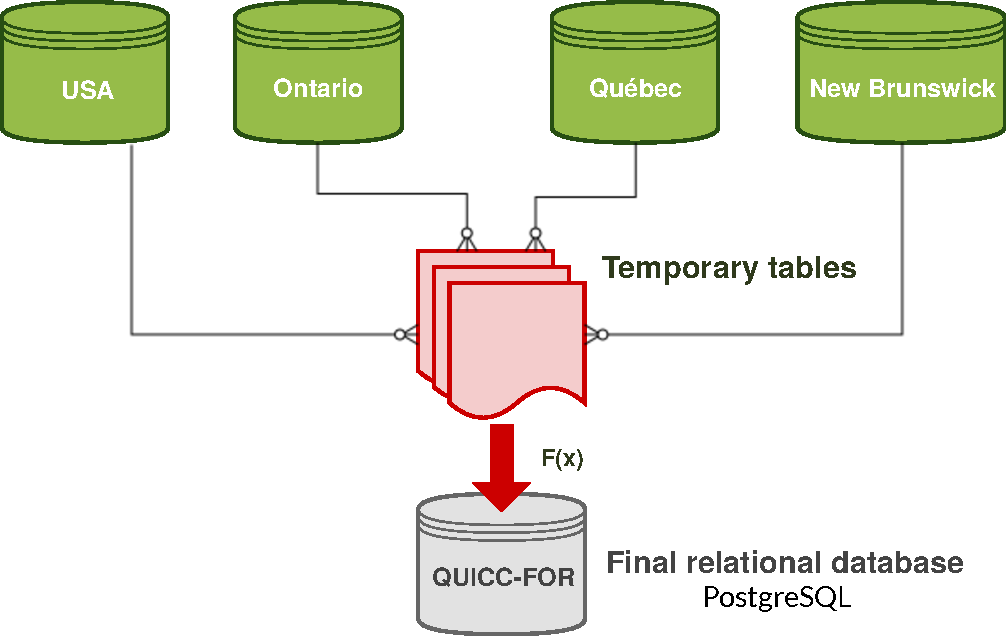
\includegraphics[width=.70\paperwidth]{Figs/quiccfor.pdf}
\end{figure}

\end{frame}

%%%%%%%%%%%%%%%%%%%%%%%%%%%%%%%%%%%%%%%%%%%%%%%%%%%%%%%%%%%%%%%%%%%%%%%%%%%%%%%%%%%%%%%%%%%%%%%%
%%% Data

\begin{frame}[t]{Data used}{Calibration}
	\vspace{-1em}
	\center \textbf{Preliminary results include only the Quebec database}
\begin{figure}
	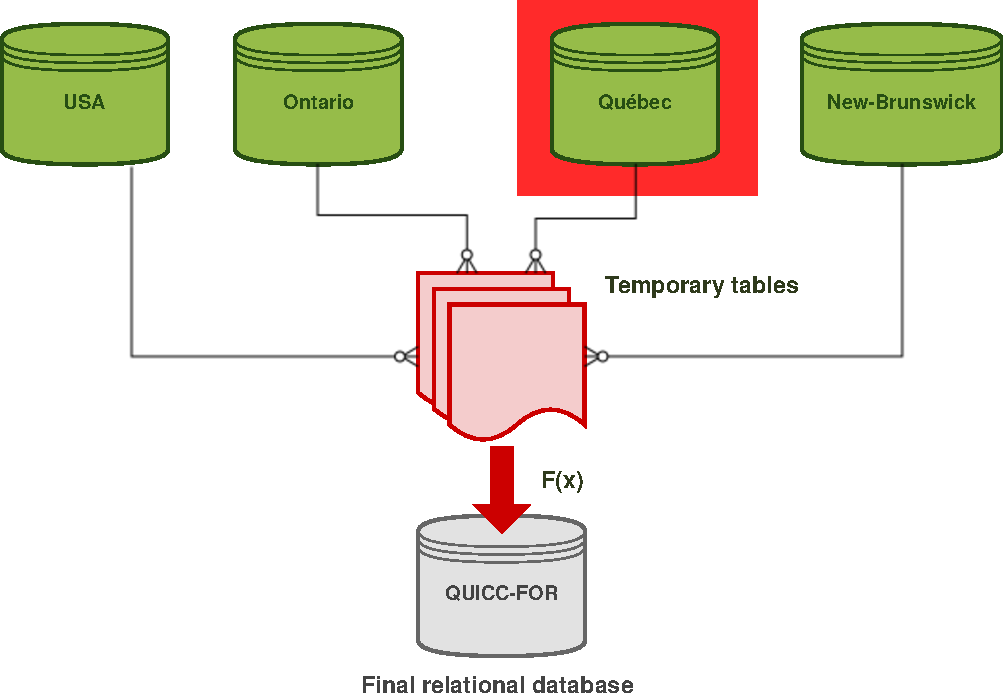
\includegraphics[width=.70\paperwidth]{Figs/quiccfor2.pdf}
\end{figure}

\end{frame}


%%%%%%%%%%%%%%%%%%%%%%%%%%%%%%%%%%%%%%%%%%%%%%%%%%%%%%%%%%%%%%%%%%%%%%%%%%%%%%%%%%%%%%%%%%%%%%%%
%%% Data

\begin{frame}{Data used}{Calibration}
	
	\begin{columns}[c]
	\begin{column}[c]{.40\paperwidth}
		\begin{figure}
			\small{Plots distribution map}
		\end{figure}
	\end{column}
	\begin{column}[l]{.50\paperwidth}

	\begin{enumerate}
			\item \textbf{Classify state of each plot}
		\begin{itemize}
			\item Plot remeasured (10 years)
			\item Transition observed between remeasurements
			\item Past-climate of the plot over 15 years
		\end{itemize}
			\item \textbf{Compute state transition probabilities} based on the past climate and neighbors plot states.
	\end{enumerate}

	\end{column}
\end{columns}

\end{frame}

%%%%%%%%%%%%%%%%%%%%%%%%%%%%%%%%%%%%%%%%%%%%%%%%%%%%%%%%%%%%%%%%%%%%%%%%%%%%%%%%%%%%%%%%%%%%%%%%
%% Explicit version 

\begin{frame}{Calibration}{Transition probabilities}

\begin{columns}[c]
	\begin{column}[c]{.40\paperwidth}

	\textbf{Figure: State transition probability function}

	\end{column}
	\begin{column}[c]{.40\paperwidth}
		
	\textbf{STM spatial explicit version}
	
	\end{column}
\end{columns}

\end{frame}


%%%%%%%%%%%%%%%%%%%%%%%%%%%%%%%%%%%%%%%%%%%%%%%%%%%%%%%%%%%%%%%%%%%%%%%%%%%%%%%%%%%%%%%%%%%%%%%%
%%% Results

\begin{frame}[t]{Results}{Actual predicted landscape}

		\begin{figure}
			\vspace{-1.5em}
			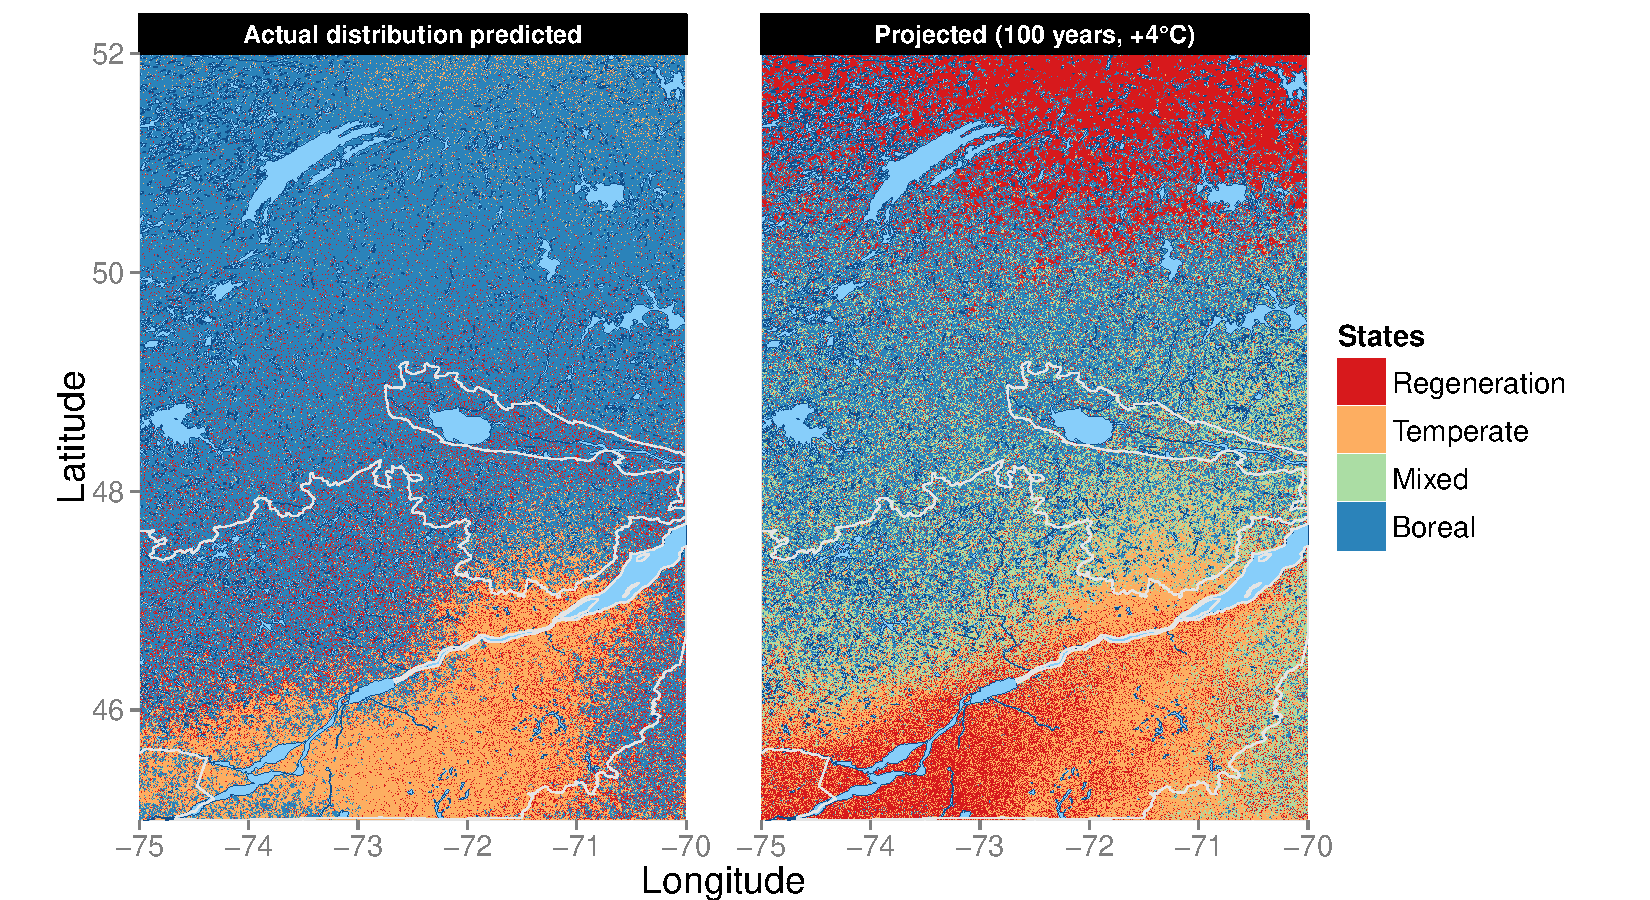
\includegraphics[height=0.79\paperheight]{Figs/outModel.pdf}
		\end{figure}

\end{frame}

%%%%%%%%%%%%%%%%%%%%%%%%%%%%%%%%%%%%%%%%%%%%%%%%%%%%%%%%%%%%%%%%%%%%%%%%%%%%%%%%%%%%%%%%%%%%%%%%
%%% Results

\begin{frame}[t]{Results}{Futur predicted landscape}

		\begin{figure}
			\vspace{-1.5em}
			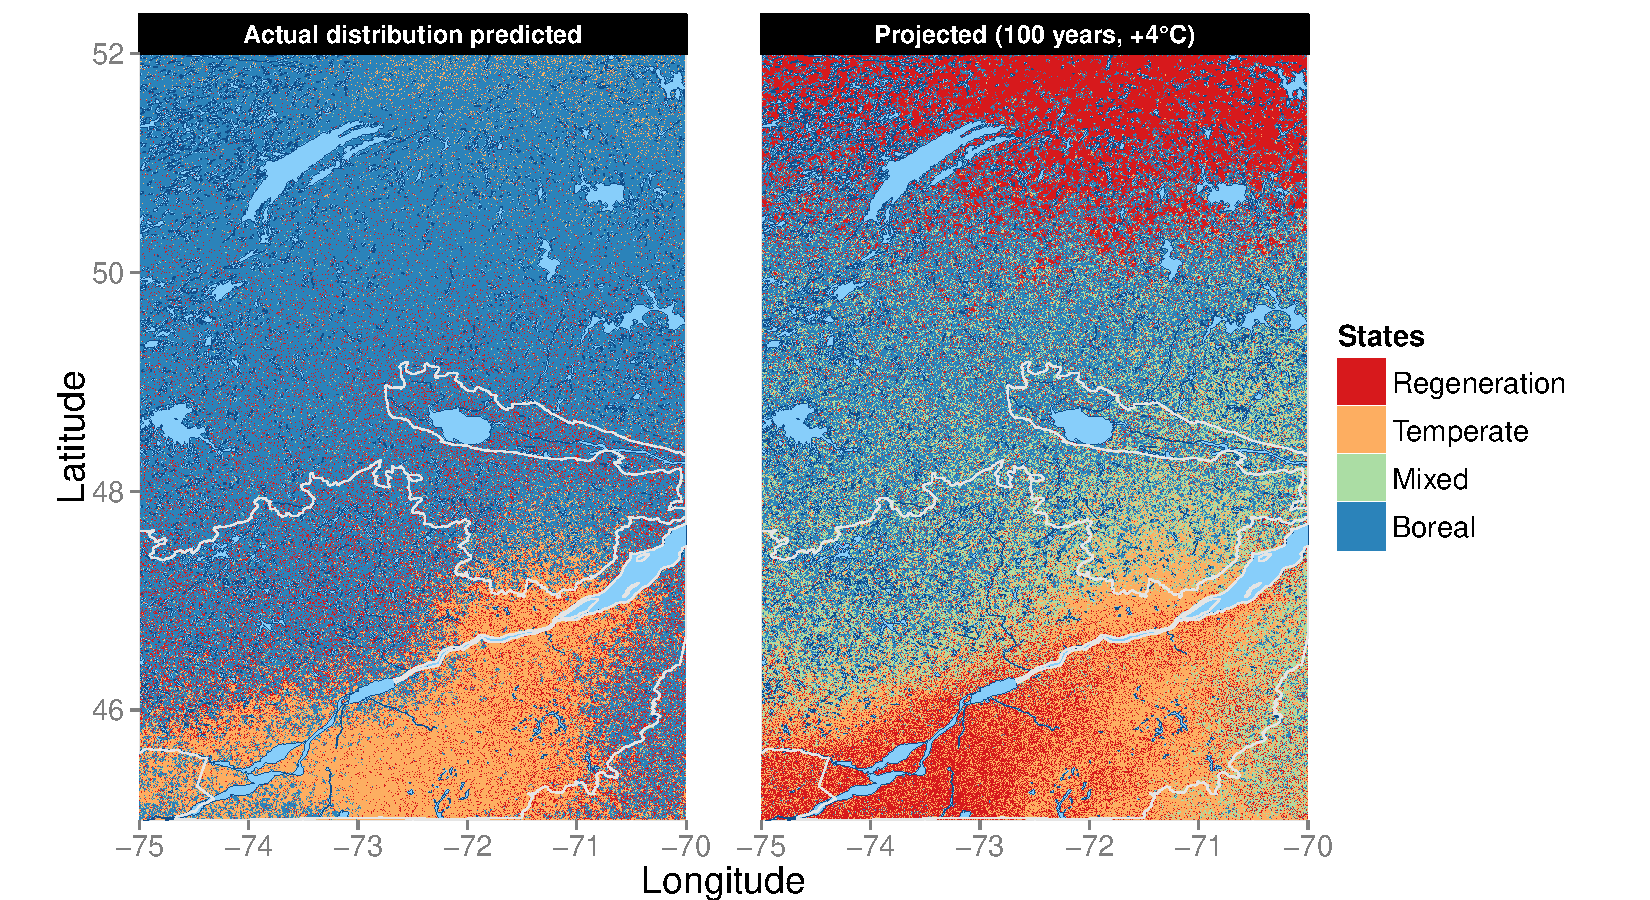
\includegraphics[height=0.79\paperheight]{Figs/outModel.pdf}
		\end{figure}

\end{frame}


%%%%%%%%%%%%%%%%%%%%%%%%%%%%%%%%%%%%%%%%%%%%%%%%%%%%%%%%%%%%%%%%%%%%%%%%%%%%%%%%%%%%%%%%%%%%%%%%
%%% Results

\begin{frame}{Incomings}

\textbf{Next steps:}
\begin{enumerate}
	\item Add all data from the QUICC-FOR database
	\item Improve the calibration
	\item Process validation 
	\item Perform simulations using Regional Climate Models (RCM)
\end{enumerate}

\end{frame}

%%%%%%%%%%%%%%%%%%%%%%%%%%%%%%%%%%%%%%%%%%%%%%%%%%%%%%%%%%%%%%%%%%%%%%%%%%%%%%%%%%%%%%%%%%%%%%%%
%%% Results

\begin{frame}[plain]{Questions}


\center{ \large
	\textbf{Thanks for your attention.} \\
	Any Questions ?}

\end{frame}

%%%%%%%%%%%%%%%%%%%%%%%%%%%%%%%%%%%%%%%%%%%%%%%%%%%%%%%%%%%%%%%%%%%%%%%%%%%%%%%%%%%%%%%%%%%%%%%%
%%% Biblio


\end{document}


%%%%%%%%%%%%%%%%%%%%%%%%%%%%%%%%%%%%%%%%%%%%%%%%%%%%%%%%%%%%%%%%%%%%%%%%%%%%%%%%%%%%%%%%%%%%%%%%
%%% Extra Slides

% 1. Paramétrisation of the model
